%!TeX jobName=challenges/web/cartopher
%\nofiles
% Created by Bonita Graham
% Last update: February 2019 By Kestutis Bendinskas
%https://es.overleaf.com/gallery/tagged/academic-journal
% Authors:
% Please do not make changes to the preamble until after the solid line of %s.

\documentclass[letterpaper,10pt]{article}
\usepackage[spanish,es-noshorthands]{babel}
\usepackage[latin1,utf8]{inputenc} % Codificación UTF-8

\usepackage[explicit]{titlesec}
\setlength{\parindent}{0pt}
\setlength{\parskip}{1em}
\usepackage{hyphenat}
\usepackage{ragged2e}
%Para colocar puntos en los itemes especiales
\usepackage{pifont}
\RaggedRight

% These commands change the font. If you do not have Garamond on your computer, you will need to install it.
%\usepackage{garamondx}
\usepackage[T1]{fontenc}
\usepackage{amsmath, amsthm}
\usepackage{graphicx}
\usepackage{caption}

% This adjusts the underline to be in keeping with word processors.
\usepackage{soul}
\setul{.6pt}{.4pt}
%This is for the color for the codign
\usepackage[dvipsnames]{xcolor}
%http://latexcolor.com/
\definecolor{almond}{rgb}{0.94, 0.87, 0.8}
\definecolor{airforceblue}{rgb}{0.36, 0.54, 0.66}
\usepackage{listings}

\lstset{
  backgroundcolor=\color{almond}, %color de fondo
  breaklines=true,
  captionpos=b,     % Establece la posición de la leyenda del cuadro de código
  basicstyle=\sffamily,
  %basicstyle=\footnotesize,
  showstringspaces=false,
  commentstyle=\color{red},
  keywordstyle=\color{blue}
}

%https://www.overleaf.com/learn/latex/Hyperlinks
%Styles and colours
\usepackage{hyperref}
\hypersetup{
    colorlinks=true,
    linkcolor=blue,
    filecolor=magenta,
    urlcolor=ForestGreen,
}
\urlstyle{same}


% The following sets margins to 1 in. on top and bottom and .75 in on left and right, and remove page numbers.
\usepackage{geometry}
\geometry{vmargin={1in,1in}, hmargin={.75in, .75in}}
\usepackage{fancyhdr}
\pagestyle{fancy}
\pagenumbering{gobble}
\renewcommand{\headrulewidth}{0.0pt}
\renewcommand{\footrulewidth}{0.0pt}

% These Commands create the label style for tables, figures and equations.
\usepackage[labelfont={footnotesize,bf} , textfont=footnotesize]{caption}
\captionsetup{labelformat=simple, labelsep=period}
\newcommand\num{\addtocounter{equation}{1}\tag{\theequation}}
\renewcommand{\theequation}{\arabic{equation}}
\makeatletter
\renewcommand\tagform@[1]{\maketag@@@ {\ignorespaces {\footnotesize{\textbf{Equation}}} #1.\unskip \@@italiccorr }}
\makeatother
\setlength{\intextsep}{10pt}
\setlength{\abovecaptionskip}{2pt}
\setlength{\belowcaptionskip}{-10pt}

\renewcommand{\textfraction}{0.10}
\renewcommand{\topfraction}{0.85}
\renewcommand{\bottomfraction}{0.85}
\renewcommand{\floatpagefraction}{0.90}

% These commands set the paragraph and line spacing
\titleformat{\section}
  {\normalfont}{\thesection}{1em}{\MakeUppercase{\textbf{#1}}}
\titlespacing\section{0pt}{0pt}{-10pt}
\titleformat{\subsection}
  {\normalfont}{\thesubsection}{1em}{\textit{#1}}
\titlespacing\subsection{0pt}{0pt}{-8pt}
\renewcommand{\baselinestretch}{1.15}

% This designs the title display style for the maketitle command
\makeatletter
\newcommand\sixteen{\@setfontsize\sixteen{16pt}{6}}
\renewcommand{\maketitle}{\bgroup\setlength{\parindent}{0pt}
\begin{flushleft}
\vspace{-.375in}
\sixteen\bfseries \@title
\medskip
\end{flushleft}
\textsc{\@author}\\
\textit{\today}
\egroup}
\makeatother

% This styles the bibliography and citations.
%\usepackage[biblabel]{cite}
\usepackage[sort&compress]{natbib}
\setlength\bibindent{2em}
\makeatletter
\renewcommand\@biblabel[1]{\textbf{#1.}\hfill}
\makeatother
\renewcommand{\citenumfont}[1]{\textbf{#1}}
\bibpunct{}{}{,~}{s}{,}{,}
\setlength{\bibsep}{0pt plus 0.3ex}

\renewcommand*{\lstlistingname}{Código}  %CAMBIA EL TITULO DE LISTING EN EL CODIGO


%%%%%%%%%%%%%%%%%%%%%%%%%%%%%%%%%%%%%%%%%%%%%%%%%

% Authors: Add additional packages and new commands here.
% Limit your use of new commands and special formatting.

% Place your title below. Use Title Capitalization.
\title{Write-up: HackTheBox - Web - Cartopher}

% Add author information below. Communicating author is indicated by an asterisk, the affiliation is shown by superscripted lower case letter if several affiliations need to be noted.
\author{Sebastián Sepúlveda @piblack}


\pagestyle{empty}
\begin{document}

% Makes the title and author information appear.
\vspace*{.01 in}
\maketitle
\vspace{.12 in}

% Start the main part of the manuscript here.
% Comment out section headings if inappropriate to your discipline.
% If you add additional section or subsection headings, use an asterisk * to avoid numbering.

\textbf{Información:} Categoria Stego, puntuacion 20.

\textbf{Descripción:} John Lennon send a secret message to Paul McCartney about the next music tour of Beatles... Could you find the message and sumbit the flag?

\section*{WriteUp}

En este desafio obtenemos una pagina que está siendo desarrrollada por hackers y queremos averiguar que hay en su pagina.

Lo que debemos hacer es una SQL Injection. Lo bueno de esto es que como la pagina está vulnerable a todo tipo de ataque sql, podemos utilizar cualquier manera, como el tipico:
\par

\texttt{
username= ’- and password= ‘\\
username= hi and password= loquesea' OR '1'='1\\
y tambien\\
username ' or 1=1-- - password=anything
}
\par

Esto nos redirije a una pagina donde estamos en el home, accedimos!

\begin{figure}[h]
  \centering
  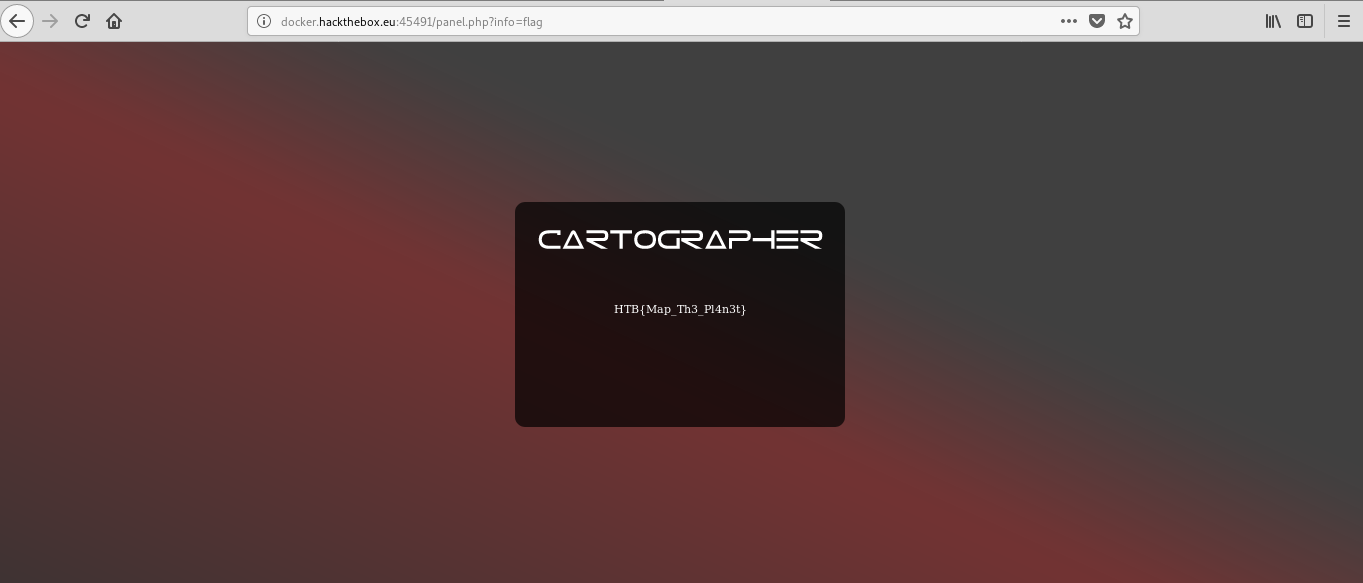
\includegraphics[scale=0.3]{images/cartopher/portada}
  \captionof{figure}{Pagina luego de ingresar}
  \label{fig:archivo}
\end{figure}

Lo unico que falta es cambiar info=home por info=flag. Eso es todo!

\begin{figure}[h]
  \centering
  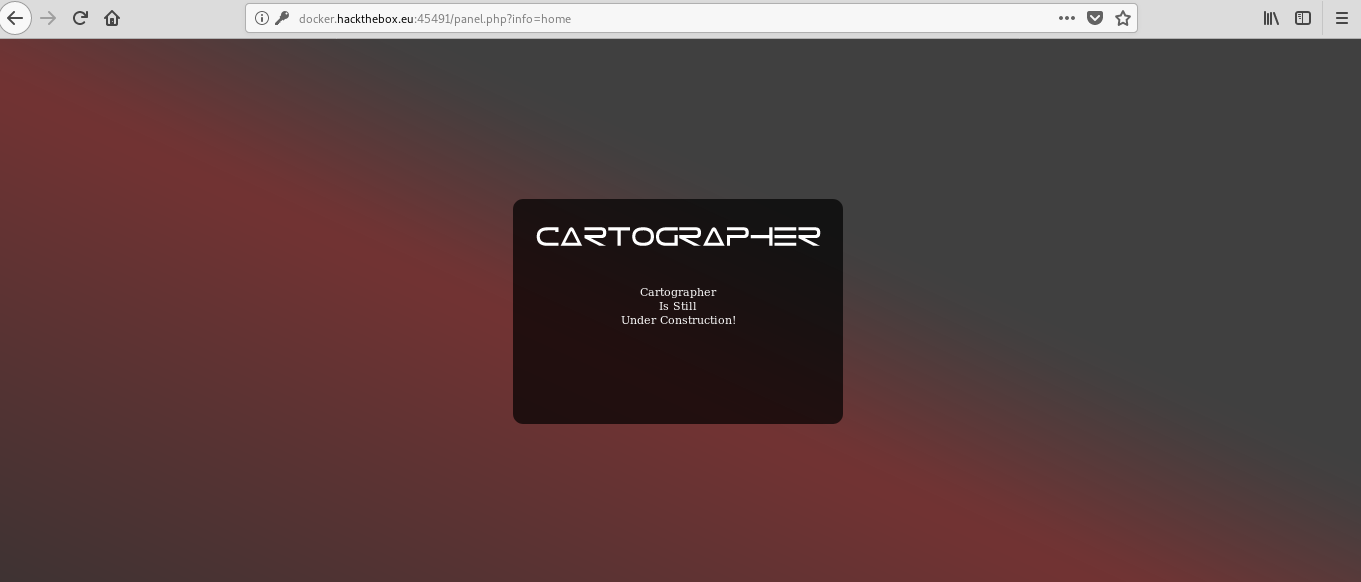
\includegraphics[scale=0.3]{images/cartopher/acceso}
  \captionof{figure}{Pagina con flag}
  \label{fig:archivo}
\end{figure}

\textbf{Flag: }HTB\{Map\_Th3\_Pl4n3t\}

\end{document}
